\documentclass{article}
\usepackage[utf8]{inputenc}

\usepackage{sectsty}
\usepackage{fancyhdr}
\usepackage[top=1.25cm, bottom=2cm, left=2cm, right=2cm]{geometry}
\usepackage{tabularx,tabulary}
\usepackage{graphicx}
\date{Mardi 26 Mars 2019}
\author{KADOCH Daoud\\LEFEVRE Sebastien}
\title{\LARGE{Rapport 3I025\\}Cahier des Charges}
\usepackage[french]{babel}
%\usepackage[utf8x]{inputenc}
%\usepackage{amsmath}
%\usepackage[colorinlistoftodos]{todonotes}
\begin{document}

\begin{titlepage}

\newcommand{\HRule}{\rule{\linewidth}{0.5mm}} % Defines a new command for the horizontal lines, change thickness here

\center % Center everything on the page
 
%----------------------------------------------------------------------------------------
%	HEADING SECTIONS
%----------------------------------------------------------------------------------------

\textsc{\LARGE Université Pierre-et-Marie-Curie}\\[3cm] % Name of your university/college
\textsc{\Large Licence Informatique 3\up{ème} Année}\\[0.5cm] % Major heading such as course name
\textsc{\large 3I025}\\[2cm] % Minor heading such as course title

%----------------------------------------------------------------------------------------
%	TITLE SECTION
%----------------------------------------------------------------------------------------

\HRule \\[0.4cm]
{ \huge \bfseries Rapport 3I025}\\[0.4cm] % Title of your document
\HRule \\[2cm]
 
%----------------------------------------------------------------------------------------
%	AUTHOR SECTION
%----------------------------------------------------------------------------------------

\begin{minipage}{0.4\textwidth}
	\begin{flushleft} \large
	\emph{Auteurs:}\\[0.2cm]
	Daoud \textsc{KADOCH}\\ % Your name
	Sebastien \textsc{LEFEVRE} % Your name
	\end{flushleft}
\end{minipage}
~
\begin{minipage}{0.4\textwidth}
	\begin{flushright} \large
	\emph{Enseignant:} \\[0.2cm]
	Nicolas \textsc{MAUDET}
	\end{flushright}
\end{minipage}\\[4cm]

%----------------------------------------------------------------------------------------
%	DATE SECTION
%----------------------------------------------------------------------------------------

{\large Mardi 26 Mars 2019}\\[3cm] % Date, change the \today to a set date if you want to be precise

%----------------------------------------------------------------------------------------
%	LOGO SECTION
%----------------------------------------------------------------------------------------

    
\includegraphics[scale=0.15]{logo_sorbonne.png} % Include a department/university logo - this will require the graphicx package
 
%----------------------------------------------------------------------------------------

\vfill % Fill the rest of the page with whitespace

\end{titlepage}

% -----------------------------------------------------
\newpage
\renewcommand{\contentsname}{\center{Table des Matières}\vspace*{5cm}}

\tableofcontents

\newpage


\section{Contexte}
	Nous étudions un jeu multijoueur où plusieurs agents se voient attribuer une fiole et doivent simplement aller la chercher par le plus court chemin possible.\\
En plus d'éviter des obstacles, les joueurs ne doivent pas rentrer en collision entre eux. \\
Pour résoudre ce problème, nous allons étudier trois solutions distinctes en comparant leurs temps d'exécution afin de déterminer laquelle de ces trois approches est la meilleure.\\
On utilisera l'algorithme "A étoile", afin de calculer le plus court chemin d'un agent à une fiole.

\section{Stratégie Opportuniste}
	\subsection{Objectif}
		Cette solution consiste au tout début, à calculer un chemin avec
		l'algorithme "a étoile" pour chacun des joueurs, une fois ceci fait, le jeu peut démarrer et chaque joueur entame son propre parcours.\\ 
L'algorithme A étoile ne gérant pas les collisions entre les joueurs, nous allons donc imposer une loi qui indique que pour chacun des joueurs J, avec C la case courante sur laquelle l'agent se trouve, si un autre joueur J' se trouve à la case C+1, alors nous recalculons un chemin A étoile à partir de la case C pour J, en considérant J' comme un mur à ce même endroit.
\begin{center}
	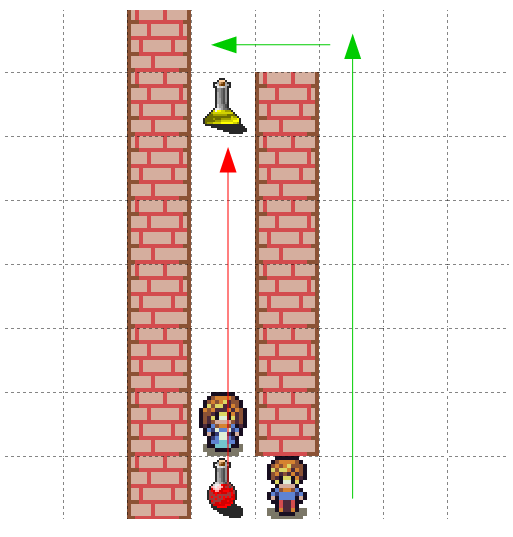
\includegraphics[scale=0.7]{Solution1_ex}
\end{center}
	Ce schéma illustre une situation dans laquelle le joueur J de case courante C (à droite de la fiole rouge) a pour chemin celui indiqué par la flèche rouge, et un autre joueur J'.\\
	Au prochain tour J' ira sur la case de la fiole rouge, pour empêcher une collision avec ce joueur, J va donc recalculer un nouveau chemin à l'aide de l'algorithme A étoile, qui est indiqué par les flèches vertes.

	
	\subsection{Implémentation}

Afin d'implémenter cette première solution, plusieurs fichiers et fonctions on été utilisés :\\

- tree\_ Class.py : Ce fichier contient une classe Tree correspondant à une structure de donnée en arbre, elle contient plusieurs fonctions :\\ 
	
- distMan : Permet de calculer la distance de Manatthan d'un nœud donné en argument, jusqu'à une case but.\\ 
	
- expansion\_ voisin : Étant donné un nœud en argument, permet d'ajouter les cases voisines, comme "enfants" de ce nœud à l'arbre courant, et renvoie la liste de ces nœuds.\\ 
	
- retropropagation : Retourne la liste des nœuds (cases) constituant le chemin de la case de départ, jusqu'à un nœud n donné en argument.\\ 
	
- min\_ f : Retourne le tuple (n,f) avec f étant minimal, de la liste donnée en argument.\\ 
	
- isInReserve : Étant donné un nœud N et une liste de nœud L, indique si N est présent dans L.\\ 
	
- etoile : Retourne une liste contenant une liste de cases, correspondant au chemin le plus court d'une case de départ, jusqu'à une case but.
	Cette fonction implémente l'algorithme "A étoile", à l'aide des fonctions déclarées précédemment.\\ 
	
	
- Solution\_ 1.py : Ce fichier correspond au Main de la solution opportuniste, elle contient les fonctions suivantes :\\ 

- conditionZone : Étant donné les coordonnées d'une case (x,y) et une liste de murs, indique par un booléen true si cette case n'est pas un obstacle ainsi que si elle n'est pas en dehors des murs, et false sinon. \\ 
	
-  predictHasNext : Étant donné un joueur J, retourne un booléen true si un joueur J' différent de J va se trouver sur la même case que J au prochain tour. \\
	
- hasNext : Cette fonction utilise la fonction predictHasNext décrite précédemment et étant donné un joueur J, retourne true si la position d'un des autres joueurs n'est pas celle que le joueur J souhaite prendre. \\ 
	
- majChemin : Cette fonction permet de recalculer un chemin A étoile à partir d'une case courante (pour ne pas repartir du début). \\ 
	
- main : Le main parcours tous les joueurs durant n itérations, et vérifie si à chaque tour, un des joueur va se retrouver en collision avec un autre au prochain tour, en utilisant les fonctions décrites précédemment. \\ 
	
	\subsection{Résultats}
		Là on expose les résultats en fonction de quelques map.
	
	
\section{Stratégie Coopérative de Base}
	\subsection{Objectif}
	
	Dans cette solution, on calcule le chemin A étoile de chaque joueur dès le début à la manière de la stratégie opportuniste, néanmoins une étape préalable devra être exécutée.\\
	En effet pour la gestion des collisions nous allons étudier le chemin de chaque joueur et déterminer quels sont les joueurs qui peuvent exécuter leurs chemin en "parallèle" en formant des groupes de passage.\\
	Afin de former ces groupes, une méthode bien particulière est employée, en effet nous parcourons chaque chemins K des joueurs, et pour chaque case C de K, si c est présente dans un des chemins des autres joueurs, alors cela signifie que ces deux joueurs risquent une collision, ils ne passeront pas ensemble.\\
	A l'inverse si K n'a pas de case en commun avec un des joueurs, alors ils feront tous deux parti du même groupe de passage.
	Lorsque les groupes de passages sont établis, les groupes de joueurs peuvent donc passer les uns après les autres sans aucuns risque de collision.
\begin{center}
	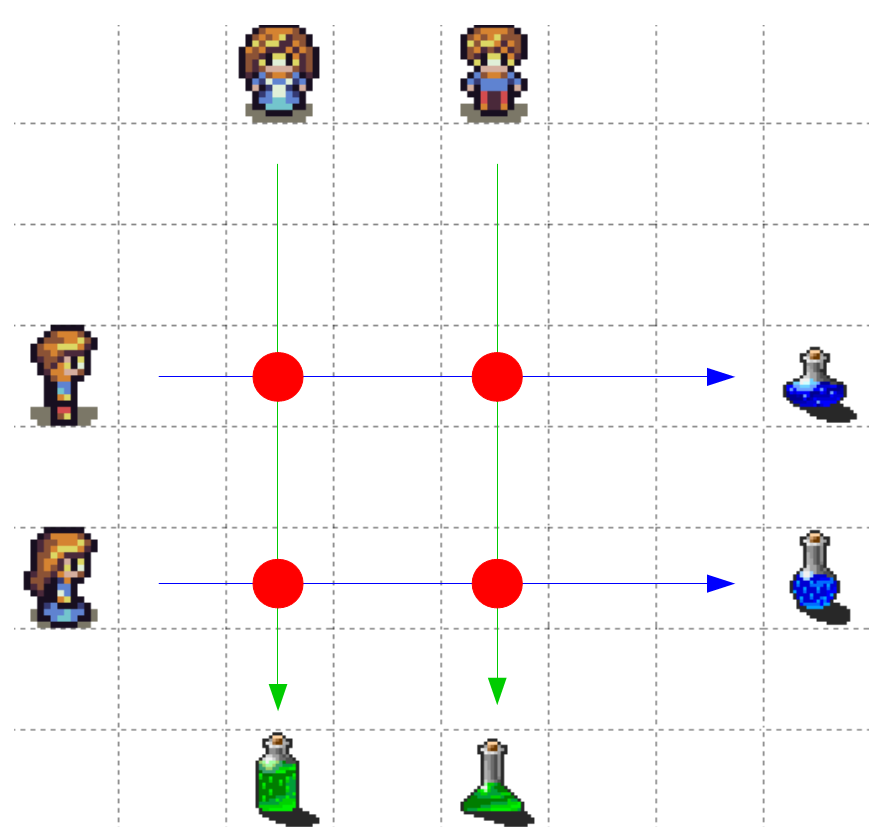
\includegraphics[scale=0.25]{Solution2_ex}
\end{center}
	
	Ce schéma illustre une situation avec quatre joueurs, nous observons ici quatre cases communes entre les joueurs qui ont été détectées par notre algorithme, représentées par les points rouges, les joueurs avec les chemins verts ne pourront pas passer avec les joueurs à chemin bleu et inversement car il y a un risque de collision.\\
	Nous pouvons donc distinguer ici deux groupes de passages : un premier groupe avec les chemins verts et un autre avec les chemins bleus.
	Si ces deux groupes passent l'un après l'autre, alors il n'y aura pas de risque de collision.\\
	
\subsection{Implémentation}

Afin d'implémenter cette première solution, plusieurs fichiers et fonctions on été utilisés : \\ 

- tree\_ Class.py : Ce fichier python est le même que décrit précédemment.\\ 

- Solution\_ 2.py : Ce fichier correspond au Main de la solution coopérative, il contient des fonctions déjà utilisées lors de la solution opportuniste, mais en contient de nouvelles : \\ 

- collision : Étant donné deux chemins (listes de cases), renvoie true si ces deux chemins possèdent au moins une case en commun, et false sinon. \\ 
	
- main : Le main implémente une liste de joueurs L, et effectue une boucle, tant que cette liste n'est pas vide (cf tant que tous les joueurs ne sont pas passés). Le joueur courant J est le premier élément L et est retiré de cette même liste, et pour chaque joueur J' restant dans la liste, si J et J' ne sont pas en collision on ajoute J' à un groupe de passage représenté par une liste. Une fois ce parcours de joueurs réalisé, on fait passer tous les joueurs du groupe de passage en même temps sans risque de collision.\\
\newpage
\section{Stratégie Coopérative avancée}

\subsection{contexte}

Après avoir implémenter ces solutions, on se demande si elles sont bien toutes viable pour toutes situations ? Sur de grandes cartes avec de larges couloir, nos algorithmes s’en sortent plutôt très bien. En revanche lorsqu’il faut traiter des problèmes de couloir où un seul et unique agent peut se déplacer dans un block de largeur. Le problème devient tout de suite différent, et  il est nécessaire de revoir les stratégies à leur base. Jusqu'à lors il n’y avait pas une réelle coopération entre les différents agents, mais seulement un moyen d’éviter les collisions. Il fallait donc implémenter une version améliorée de l’algorithme A* pour parvenir à pallier ces problèmes . Pour se faire il a fallut effectuer une recherche plus ou moins exhaustive des différents cas ou l’algorithme de base posait problème.

\subsection{Résolution de probleme}


\noindent 1 - Comment éviter de prendre un tout autre chemin beaucoup plus long à cause de la rencontre d’un autre agent ?

\noindent 2 - Comment faire en sorte qu’un agents puisse effectuer une pause à un instant donné afin de laisser passer certains autres agents lorsqu'il s'agit de la seul solution possible?


\begin{figure}[h]
   \begin{minipage}{0.5\textwidth}
     \centering
     \includegraphics[width=.7\linewidth]{s2}
     \caption{problème 1 }\label{Fig:1}
   \end{minipage}\hfill
   \begin{minipage}{0.5\textwidth}
     \centering
     \includegraphics[width=.7\linewidth]{s1}
     \caption{problème 2}\label{Fig:2}
     \end{minipage}
\end{figure}

\begin{figure}[h]
     \centering
     \includegraphics[width=.2\linewidth]{s2_2}
     \caption{problème 2}\label{Fig:3}
\end{figure}
Il fallait donc ajouter une composante temporelle pour pallier ces problèmes, et passer sur une recherche de chemin à base de réservations de case par les  agents à des instant t précis. En ajoutant cette composante, les agents peuvent désormais s’attacher au parcours des autres agents, pas dans leur globalité mais uniquement à certains instants. Ceci permet donc à un agent de rechercher des emplacements d’évitement (lorsqu’il ne peut pas continuer sur son chemin). Ceci l'amène à coopérer avec les autres agents et avoir un coup de chemin qui peut être parfois drastiquement réduit comme on peut le voir sur la figure 1. Dans la figure 2 et 3 il est primordiale de passer par cette méthode car pour les deux agents il s'agit de leur seul et unique cheveux possible.
\\

\newpage

\subsection{Autres Approches}
D’autres problèmes on été mis en jeu notamment, lorsqu’un agent a fini son parcours et se trouve donc à l’emplacement de sa fiole. Que devient il ?\\

Nous avons décidé qu’il deviendrait un mur et qu’il soit considéré tel quel par les autres agents que à partir du moment où il parvient à son but. Il a fallu ajouter à cela un autre dictionnaire référençant les positions finales t de chaque agent, traiter différemment le choix de case à chaque étape et que lorsqu’un un agent souhaite accéder à cette case après cet instant t, il n’aura désormais plus le droit. 
\\
\begin{center}
	\includegraphics[scale=0.4]{s4}
\end{center}

Cependant en ajoutant cette dernière spécificité un nouveau problème beaucoup plus complexe se joue. En effet, lorsqu’un agent est considéré comme un obstacle après être arrivé à sa position finale, pourrait-il bloquer d’autres agents dans leur recherche de chemin (si celui ci était à sens unique) ? Oui et cela est un gros problème. Chercher à pallier ce problème est très complexe car il fait intervenir beaucoup d’incertitudes dans le calcul de chemin. \\

\begin{center}
	\includegraphics[scale=0.3]{s5}
\end{center}

Une première idée était de détecter les agents qui se retrouvaient bloqués dans la construction de leur chemin en admettant un pallier en terme d’itérations (pas très propre mais semble être la meilleure solution) une fois ces agents détectés, il faut faire en sorte que tout autre agents qui essaye d’accéder aux cases d’un agent dit « en fuite » doivent attendre qu’il passe, en considérant ces cases comme des obstacles temporaires jusqu'à à instant t.

\end{document}